
%%%
% Any line that begins with a percent symbol is a comment. To compile
% this document and view the output:
%
% Run Latex
% Run Bibtex
% Then run Latex twice.
%
% This should produce the output PDF file named main.pdf
%%%

% This defines the style to use for this document.
% Do not modify.
\documentclass[letterpaper]{article}

% The following are akin to "import" statements in Python or Java -
% these import useful commands into the document for you to use.  You
% don't have to modify any of these lines. The AAAI package formats
% this document in the style of submissions to the American
% Association for Artificial Intelligence conference, one of the top
% AI conferences in the world. You will find that many academic
% publications in AI use this format.
\usepackage{aaai} 
\usepackage{times} 
\usepackage{helvet} 
\usepackage{courier} 
\setlength{\pdfpagewidth}{8.5in} 
\setlength{\pdfpageheight}{11in} 
\usepackage{amsmath}
\usepackage{amsthm}
\usepackage{amssymb}
\usepackage{graphicx}
\usepackage{graphics}
\usepackage{moreverb}
\usepackage{subfigure}
\usepackage{epsfig}
\usepackage{txfonts}
\usepackage{palatino}
\usepackage{algpseudocode}
\usepackage{multirow, multicol}
\usepackage{url}
\usepackage{tablefootnote}
\usepackage{color}

\setcounter{secnumdepth}{1}
\nocopyright

% Fill in your paper title, names and emails below
% The "\\" is used to break lines. The \url command
% is useful for typesetting URLs and email addresses (it uses the
% Courier font).
\title{Course Scheduling as a Constraint Satisfaction Problem}
 \author{Micah Brown \and Ben Wiley\\
 \url{{msbrown,bewiley}@davidson.edu}\\
 Davidson College\\
 Davidson, NC 28035\\
 U.S.A.}

% This is the "true" start of the document. All the text in your
% write-up should be placed within the \begin{document} and
% \end{document} decorators.
\begin{document}

\maketitle % formats the title nicely, do not modify

% While at this point you could just begin your write-up, often, it's
% useful to write each section of your write-up in a separate tex
% file (not unlike the modular decomposition you do for code you
% write). These \input commands insert the contents of the
% specified tex files in the order specified. Every write-up you
% submit must contain the following sections, in the shown order. Open
% each of the indicated tex files to understand what goes in each
% section, as well as for more TeX tips.

% Place the contents of your abstract between the
% \begin{abstract} and \end{abstract} decorators.

\begin{abstract}

The current system for selecting courses at Davidson College is known as
``Webtree''. Webtree selects courses for students, in order of class
seniority, in a random order within their class. This outdated system has been
in place for decades, and is very static. We attempt to redesign
Webtree such that it selects courses for students in a more efficient
way. By framing the problem as a constraint satisfaction problem, we
have created a more optimal solution to assigning courses than the
current system. 

% The \textbf{} command makes the specified text bold. The \emph{} or
% \textit{} command are used to italicize text. In general, text is never
% underlined.

% DON'T FORGET TO MATCH EACH OPEN BRACE WITH A CLOSING BRACE!
\end{abstract}



% The \section{} command formats and sets the title of this
% section. We'll deal with labels later.
\section{Introduction}
\label{sec:intro}

With over 400 courses offered every semester at Davidson College,
assigning students courses based on their preferences is not a trivial
task. For years, the Office of the Registrar has used ``Webtree'', a
system designed to be fair yet give students preferential treatment
according to seniority. Webtree, untouched in the past several decades, remains a constant
source of confusion, and later in the course selection process,
frustration. At first, students are overwhelmed by the non-intuitive
user interface. Once Webtree has run, students are then disappointed
by the courses they receive. Due to the static nature of Webtree, it
is not uncommon for students to receive only one or two courses after
an entire run of Webtree (with four courses being a full
course-load). 

Course scheduling is a common problem for artificial intelligence
researchers and much work has gone into efficient ways to assign
courses. However, Davidson College's Webtree is a unique problem that
has not been studied yet, to our knowledge. Much of the prior research
into course scheduling involves placing courses in appropriate
classrooms and at appropriate times. Davidson College's course
selection is unique because course ceilings are strictly enforced, to
ensure that class enrollment sizes are kept small to give students the
necessary attention to foster a positive learning
environment. Additionally, room selection is rarely an issue at
Davidson College because very few classes exceed an enrollment of $30$
students, and so most classes can fit into most rooms.

Recently, researchers have been framing the university course
selection problem as a constraint satisfaction problem
\cite{darden}. Constraint satisfaction problems maximize or minimize
an objective function over a set of constraints with variables in a
given domain. By setting constraints as actual limitations that exist,
such a course must obey the given course ceiling, the course
scheduling process can be made equitable and processed quickly.
 
The rest of the paper is organized...

% Citations: As you can see above, you create a citation by using the
% \cite{} command. Inside the braces, you provide a "key" that is
% uniue to the paper/book/resource you are citing. How do you
% associate a key with a specific paper? You do so in a separate bib
% file --- for this document, the bib file is called
% project1.bib. Open that file to continue reading...

% Note that merely hitting the "return" key will not start a new line
% in LaTeX. To break a line, you need to end it with \\. To begin a 
% new paragraph, end a line with \\, leave a blank
% line, and then start the next line (like in this example).
%Overall, the aim in this section is context-setting: what is the
%big-picture surrounding the problem you are tackling here?



\section{Background}
\label{sec:background}

The current system of course selection, Webtree, was designed to allow
students to customize their course selections to deal with various
contingencies. For example, a student might want a different second
course option depending on whether or not he or she successfulling
recieved his or her first option. Webtree consists of three binary trees (depth
of $3$), which are traversed according to an elaborate
algorithm. Students' fourth class is ranked in order $1-4$, and is
selected according to availability in that order. For a visual
represention of Webtree, as well a chance to imagine the confusion that
many students feel when filling it out, see
Figure~\ref{fig:webtr}. Interested readers are referred to the
Davidson College Registrar's Office for a detailed description of the
Webtree algorithm\footnote{http://www.davidson.edu/offices/registrar/course-registration-and-webtree/how-to-use-webtree}.

\begin{figure}[htb]
  \centering  % centers the image in the column
  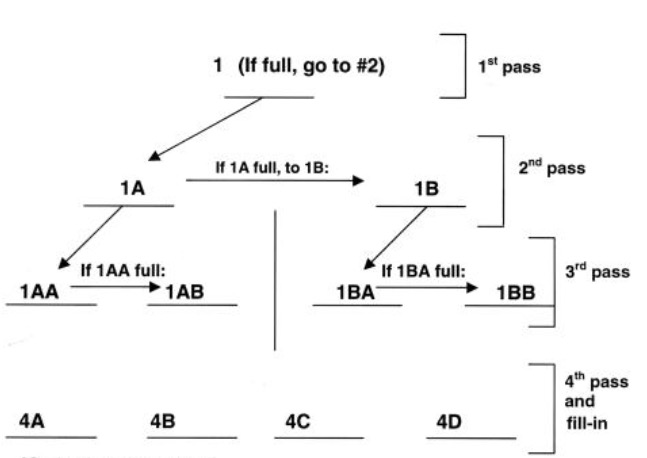
\includegraphics[width=0.37\textwidth]{figs/webtree.jpg}
  % *Every* figure should have a descriptive caption.
  \caption{The complicated nature of Davidson College's Webtree. Image
    courtesy of Davidson College Registrar.}
  \label{fig:webtr}
\end{figure}

Alternatively, we chose to approach this problem as a constraint
satisfaction problem. A constraint satisfaction problem takes the
inputs $Varibles$, $Domains$, and $Constraints$ \cite{aima}. We chose to
specifically implement this problem as a psuedoboolean constraint
satisfaction problem. A psuedoboolean problem has its domain limited
to {True, False}, or {0,1}. Thus, we set up our problem as a set of
constraints of inequalities, and an objective function that we attempt
to minimize. Several computer scientists have devoted time to creating
psuedoboolean solvers and allowing the public to have full access to
them.

To determine whether one method of scheduling is ``better'' than
another, we must devise a way of ranking a schedule. Since we are
given preferences in Webtree format, we must be able to assign an
individual request a certain rank. For our purposes, we have defined
rank of a scheduling assignment to be the sum of ranks of all the
courses assigned in that given assignment: \begin{equation}\label{rank}Rank_{scheduling} =
  \sum_{i=0}^{|Variables|}{rank(i)*x_i}\end{equation} 

A course is assigned a given rank depending on the tree and branch
that it was placed in the original Webtree. If a request was in the
first ``branch'' (i.e. the root node of a Tree), then the course is given
a rank {1-4}, according to which Tree it is in. For Trees {1-3}, the
rest of the courses are then ranked according to whether they are a
left child or a right child. Left children are a higher priority than right
children and given a rank of 1; right children are the second option
and thus given a rank of 2. Requests on Tree 4 are ranked {4-7}, in
the order that they are placed.





\section{Experiments}
\label{sec:expts}

In this section, you should describe your experimental setup. What
were the questions you were trying to answer? What was the
experimental setup (number of trials, parameter settings, etc.)? What
were you measuring? You should justify these choices when
necessary. The accepted wisdom is that there should be enough detail
in this section that I could reproduce your work \emph{exactly} if I
were so motivated.


\section{Results}
\label{sec:results}

% Present the results of your experiments. Simply presenting the data is
% insufficient! You need to analyze your results. What did you discover?
% What is interesting about your results? Were the results what you
% expected? Use appropriate visualizations. Prefer graphs and charts to
% tables as they are easier to read (though tables are often more
% compact, and can be a better choice if you're squeezed for space).
% \textbf{Always} include information that conveys the uncertainty in
% your measurements: mean statistics should be plotted with error bars,
% or reported in tables with a $\pm$ range. The $95\%$-confidence
% interval is a commonly reported statistic.

The results from our experiment are summarized in Table ~\ref{fig:mainresults}.
\begin{table}[h]
\begin{tabular}{lllll}
 & \begin{tabular}[c]{@{}l@{}}Min.\\ courses\end{tabular}
 & \begin{tabular}[c]{@{}l@{}}Avg. \\ rank\end{tabular}
 & \begin{tabular}[c]{@{}l@{}}Avg.\\ courses\\ granted\end{tabular}
 & \begin{tabular}[c]{@{}l@{}}Students\\ with 4\\
     courses \end{tabular} \\ \\
\begin{tabular}[c]{@{}l@{}}Webtree\\
  \\\end{tabular}& \begin{tabular}[c]{@{}l@{}}N/A \\ \\\end{tabular}
 & \begin{tabular}[c]{@{}l@{}}-6.30\\ \\\end{tabular}
 &\begin{tabular}[c]{@{}l@{}}3.74\\ \\\end{tabular}
 & \begin{tabular}[c]{@{}l@{}}1396\\ \\\end{tabular} \\ 
\begin{tabular}[c]{@{}l@{}}CSP\\ \\\end{tabular}
 & \begin{tabular}[c]{@{}l@{}}0\\ \\\end{tabular}
 & \begin{tabular}[c]{@{}l@{}}-6.47\\ \\\end{tabular}
 &\begin{tabular}[c]{@{}l@{}}3.72\\ \\\end{tabular}
 & \begin{tabular}[c]{@{}l@{}}1440\\ \\\end{tabular} \\ 

\begin{tabular}[c]{@{}l@{}}CSP\\ \\\end{tabular}
 & \begin{tabular}[c]{@{}l@{}}2\\ \\\end{tabular}
 & \begin{tabular}[c]{@{}l@{}}-6.46\\ \\\end{tabular}
 &\begin{tabular}[c]{@{}l@{}}3.72\\ \\\end{tabular} & \begin{tabular}[c]{@{}l@{}}1427\\ \\\end{tabular} \\ 

\begin{tabular}[c]{@{}l@{}}CSP\\ \\\end{tabular}
 & \begin{tabular}[c]{@{}l@{}}3\\ \\\end{tabular}
 & \begin{tabular}[c]{@{}l@{}}-6.43\\ \\\end{tabular}
 &\begin{tabular}[c]{@{}l@{}}3.75\\ \\\end{tabular} & \begin{tabular}[c]{@{}l@{}}1354\\ \\\end{tabular} \\ 

\end{tabular}
\caption{Our results of course assignment, compared to Webtree as a
  control. CSP stands for Constraint Satisfaction Problem, the method
used in this experiment.}
\label{fig:mainresults}
\end{table}




% \subsection{Embedding Pictures}
% \label{subsec:pics}

% See the source code (\texttt{results.tex}) for instructions on how to
% insert figures (like figure~\ref{fig:tex}) or plots into your
% document.


% \begin{figure}[htb]

%   \centering  % centers the image in the column

%   % replace the second argument below with your filename. I like to
%   % place all my figures in a sub-directory to keep things organized
%   \includegraphics[width=0.37\textwidth]{figs/file_extensions.png}

%   % *Every* figure should have a descriptive caption.
%   \caption{On the trustworthiness of \LaTeX. Image courtesy of \texttt{xkcd}.}

%   % The label is a handle you create so that you can refer to this
%   % figure (using the \ref{} command) from other parts of your
%   % document. LaTeX automatically renumbers figures and updates
%   % references when you recompile, so you should do it this way rather
%   % than hard-coding in references. Notice that I've also been
%   % creating labels for the various sections in the document; I could
%   % use \ref{} command to refer to those sections using their labels
%   % too.
%   \label{fig:tex}

% \end{figure}



\section{Conclusions}
\label{sec:concl}

This study sought to establish a novel method for assigning courses at
Davidson College by framing the problem as a constraint satisfaction
problem. After a comparative analysis of the old system of Webtree and
our new method, using a pseudoboolean SAT solver, we conclude that our
solution assigns courses in a manner that gives more students all four
courses (i.e. a full course-load), while giving all students more
courses that they want than Webtree does. Our best end state was
obtained in the absence of the additional constraint on minimum number
of courses granted for each student. Without this state, our model
performs better than Webtree by providing a just and appealing
distribution of courses for all students. Therefore, if an overhaul to
the method of assigning courses at Davidson College is in the near
future, framing it as a constraint satisfaction problem should be a
strong consideration of the Office of the Registrar. 


Future research should establish a new method and interface for
ranking courses. It should be simplified from the current state, while
still giving students a chance to customize different contingencies
depending on whether or not they receive certain courses. Importantly, more
research should examine what sorts of additional constraints or constraint
modifications could result in improved scheduling, as well as suitable ways to
incorporate desired hierarchical schemas such as class and lottery number. Does
there exist a constraint schema that can supply a higher number of completed
schedules than vanilla Webtree, while simultaneously returning a higher number
of fulfilled requests and a higher score of course satisfaction?


\section{Acknowledgements} 
\label{sec:ack} 

Thanks to Jackson Spell for his tip on using pseudobooleans.


% This creates the references section. Open the project1.bib file to
% see how to organize your references.
\bibliography{project1}
\bibliographystyle{aaai} % sets citation and bib style, do not modify

\end{document}
